% This is LLNCS.DOC the documentation file of
% the LaTeX2e class from Springer-Verlag
% for Lecture Notes in Computer Science, version 2.4
\documentclass{llncs}
\usepackage{llncsdoc}
%
\usepackage{graphicx}

\usepackage[pageanchor=true,hidelinks]{hyperref}
\usepackage{color}
\definecolor{mygray}{rgb}{0.6,0.6,0.6}
\definecolor{lightgray}{rgb}{0.92,0.92,0.92}
\definecolor{darkgreen}{rgb}{0,0.7,0}

% Great package for spaces in commands
\usepackage{xspace}

% for footnotes in tables
\usepackage{tablefootnote}

% for title caps
\usepackage{titlecaps}
\Addlcwords{and, the, or, of, that, our, by, a, prevent, for}

% default options for listings
\usepackage{listings}
\usepackage{listingsutf8}
\usepackage{textcomp}     % access \textquotesingle
\lstset{
	backgroundcolor=\color{lightgray},
	basicstyle=\scriptsize{}\ttfamily,
	breaklines=true, 
	captionpos=b,
	commentstyle=\color{darkgreen}, 
	frame=single,
	keywordstyle=\color{blue}, 
	numbers=left,
	numbersep=5pt,
	numberstyle=\tiny\color{mygray},
	rulecolor=\color{black},
	showstringspaces=false,
	upquote=true,
	belowskip=-6ex,
}


\newcommand{\dq}[1]{``{#1}''}
%% THIS IS THE DATA FOR OUR THESIS, UPDATING HERE WILL UPDATE EVERYWHERE %%
\newcommand{\urls}{23,553,796\xspace}

\newcommand{\forms}{7,354,425\xspace}
\newcommand{\formsDelta}{31.22\%\xspace}

\newcommand{\emailforms}{1,228,774\xspace}
\newcommand{\emailformsDelta}{16.71\%\xspace}

\newcommand{\fuzzed}{1,012,530\xspace}
\newcommand{\fuzzedDelta}{82.40\%\xspace}

\newcommand{\recd}{74,192\xspace}
\newcommand{\recdDelta}{7.33\%\xspace}

\newcommand{\diffFoundFuzz}{9,682\xspace}
\newcommand{\malfuzzed}{64,510\xspace}
\newcommand{\malfuzzedDelta}{86.95\%\xspace}

\newcommand{\success}{994\xspace}
\newcommand{\successDelta}{1.54\%\xspace}
\newcommand{\successWebsitesDelta}{0.038\%\xspace} % calc domains/total_domains 414/1,085,365

\newcommand{\slowSelenium}{31.58\%\xspace}
\newcommand{\slowParse}{11.05\%\xspace}

\newcommand{\domains}{414\xspace}
\newcommand{\ips}{604\xspace}

\newcommand{\emailedDefaultmailbox}{113\xspace}
\newcommand{\responses}{21\xspace}
\newcommand{\confirmed}{15\xspace}


\newcommand{\ipsblacklist}{157\xspace}
\newcommand{\ipsblacklistmulti}{46\xspace}

\newcommand{\ehibcc}{583\xspace}
\newcommand{\ehixcheck}{493\xspace}
\newcommand{\ehito}{229\xspace}
\newcommand{\ehibccxcheck}{310\xspace}
\newcommand{\ehitoxcheck}{15\xspace}
\newcommand{\ehinuserxcheck}{239\xspace}
\newcommand{\ehiuniquenuserxcheck}{182\xspace}

% these refer to unique domains, not unique forms
\newcommand{\uniqueforms}{1,085,365\xspace}
\newcommand{\uniqueemailforms}{198,306\xspace}

\newcommand{\totalattachmentcount}{2,950\xspace}
\newcommand{\totalvirusattachmentcount}{265\xspace}
\newcommand{\totalvirusemails}{443\xspace}

\newcommand{\ehi}{E-\nobreak{}mail Header Injection\xspace}
\newcommand{\emails}{\email{}s\xspace}
\newcommand{\emailed}{\email{}ed\xspace}    
\newcommand{\Email}{E-\nobreak{}mail\xspace}        
\newcommand{\Emails}{\Email{}s\xspace}



\begin{document}
	
\title{Measuring E-Mail Header Injections on the World Wide Web}


\author{
	Sai Prashanth Chandramouli\inst{1}
	\and Pierre-Marie Bajan\inst{2}
	\and Christopher Kruegel\inst{3}
	\and Giovanni Vigna\inst{3}
	\and Ziming Zhao\inst{1}
	\and Adam Doup\'e\inst{1}
	\and Gail-Joon Ahn\inst{1}
	}

\institute{
	Arizona State University\\
	\email{\{saipc, zzhao30, doupe, gahn\}@asu.edu}
	\and IRT SystemX\\
	\email{pierre-marie.bajan@irt-systemx.fr}
	\and University of California, Santa Barbara\\
	\email{\{chris, vigna\}@cs.ucsb.edu}
	}

\renewcommand{\email}{e-\nobreak{}mail\xspace}
\maketitle

\vspace{-2.5ex}
\begin{abstract}
	\ehi vulnerability is a class of vulnerability that can occur in
    web applications that use user input to construct \email messages.
    \ehi vulnerabilities exist in the built-in \email functionality of
    the popular languages PHP, Java, Python, and Ruby. With the proper
    injection string, this vulnerability can be exploited to allow an
    attacker to inject additional headers, modify existing headers,
    and alter the content of the \email.

	While \ehi vulnerabilities are known to the community, and some
    commercial vulnerability scanners claim to discover \ehi
    vulnerabilities, they have never been studied by the academic
    community. This paper presents a scalable mechanism to
    automatically detect \ehi vulnerabilities and uses this mechanism
    to quantify the prevalence of \ehi vulnerabilities on the web.
    From crawling \urls URLs, we found \success vulnerable URLs across
    \domains domains. 135 of these domains are in the Alexa top 1
    million, and five of them are in the top 20,000. 137 of the
    vulnerable domains are using anti-spoofing mechanisms such as
    DKIM, SPF, or DMARC, and \ehi renders this protection useless.
    This work shows that \ehi vulnerabilities are widespread and
    deserve future research attention.
\end{abstract}


\section{Introduction}\label{sec:Introduction}

The World Wide Web has single-handedly brought about a change in the way we use computers. The ubiquitous nature of the web makes it possible for anyone to access information and services anywhere and on multiple devices such as phones, laptops, TVs, and cars. This access has ushered in an era of web applications which depend on user input.
While the rapid pace of development has improved the speed of
information dissemination, it comes at a cost. As users move more and
more of their personal and financial information to web applications,
attackers are responding by using web application vulnerabilities to steal lucrative data.

Many common and well-known web application vulnerabilities, such as SQL Injection and Cross-Site Scripting~\cite{OWASPT10}, are command injection vulnerabilities~\cite{commandinjection}, where malicious user input is used to alter the structure of a command (SQL query and JavaScript code respectively). Developers of web applications must use the correct sanitization routine in all paths from user input to a command. 

\ehi vulnerabilities are a lesser-known command injection vulnerability. We verified that this vulnerability exists in the implementation of the built-in \email functionality in the popular languages PHP, Java, Python, and Ruby. The format of \email messages is defined by the Simple Mail Transfer Protocol (SMTP)~\cite{rfc5322}. Each \email message is represented by a series of headers separated by newlines, followed by the body content (separated from the headers by two newlines). Some of these headers are mandatory (\lstinline{From}, \lstinline{To}, \lstinline{Date}), but the headers could also include other information such as the \lstinline{Subject}, \lstinline{BCC}, etc.

With the proper exploit injection string, \ehi vulnerabilities can be exploited by an attacker to inject additional headers, modify existing headers, or alter the contents of the \email---while still appearing to be from a legitimate source. \ehi exploits allow an attacker to perform \email spoofing, resulting in phishing attacks \emph{that are sent from the actual \email server}, and thus bypass \email spoofing technologies, such as DKIM~\cite{allman2007domainkeys}, SPF~\cite{schlitt2006sender}, and DMARC~\cite{kucherawy2015domain}.

While some command injection vulnerabilities have received extensive attention from the research community, \ehi vulnerabilities have received little focus. In fact, the Acunetix vulnerability scanner contains an AcuMonitor component which claims to detect \ehi vulnerabilities while scanning~\cite{acumonitor}. Unfortunately, as a commercial product, little is known about how AcuMonitor detects \ehi vulnerabilities. 

To shed light on this little-studied vulnerability class, we describe
\ehi vulnerabilities and measure \ehi vulnerabilities. To perform this
measurement, we crawled the web, extracted forms with \email fields,
and injected them with different payloads to infer the existence of an
\ehi vulnerability. We then automatically audited received \emails to
see if any of the injected data was present. This allowed us to
classify whether a particular URL was vulnerable to the attack. Our
automated system works in a black-box manner, without looking at the
web application's source code, and only analyzes the payloads in the
\emails.\\\\

In summary, we make the following contributions:
\begin{itemize}

\item We develop a black-box approach to detect \ehi vulnerabilities in a web application.

\item We develop an open-source system to crawl the web and automatically detect \ehi vulnerabilities.

\item We use our system to crawl \urls URLs, and we find \success URLs vulnerable to \ehi across \domains domains. 

\item We perform detailed analyses on the domains found to be vulnerable: finding their Alexa rankings, the technologies used in such vulnerable domains, presence of \email spoofing protection, presence of such domains on existing spam-lists, and the ability to send malicious attachments.

\end{itemize}


\section{Background}
\vspace{-2.5ex}
\ehi belongs to the class of command injection vulnerabilities. However, unlike its more popular siblings, SQL injection~\cite{sql1,sql0,sql2}, Cross-Site Scripting~\cite{Injection1,KleinAmit}, or HTTP Header Injection~\cite{sessionride}, relatively little research is available on \ehi vulnerabilities.

As with other command injection vulnerabilities, \ehi is caused by
improper or nonexistent sanitization of user input. If the program
constructs \emails from user input and fails to check for the presence
of \email headers, a malicious user can control the headers of this particular e-mail. \ehi vulnerabilities can be leveraged to enable malicious attacks, including, but not limited to, spoofing or phishing.

\subsection{History of \ehi}

\begin{lstlisting}[language=PHP,caption={PHP program with e-mail
      header injection vulnerability.},label={code:phpemi}, float]
$from = $_REQUEST['email'];
$subject = 'Hello XYZ';
$message = 'We need you to reset your password';
$to = 'xyz@example.com';
$retValue = mail($to, $subject, $message, "From: $from");
\end{lstlisting}



\begin{table}[tbp]
  \scriptsize
	\centering
	\begin{tabular}{|c|p{5.5cm}|c|}
		\hline
		\multicolumn{1}{|c|}{\textbf{CVE No.}} & 
		\multicolumn{1}{c|}{\textbf{Affected Software}} &
		\multicolumn{1}{c|}{\textbf{Year}}\\
		\hline
		{2002-1575} & {cgiemail} & {2004}\\
		\hline
		{2002-1771} & {FormMail 1.9} & {2005}\\
		\hline
		{2002-1917} & {Geeklog 1.35} & {2005}\\
		\hline
		{2005-0493} & {Biz Mail Form <=2.2} & {2005}\\
		\hline
		{2005-2854} & {thesitewizard.com} & {2005}\\
		\hline
		{2005-3883} & {PHP mb\_send\_mail} & {2005}\\
		\hline
		{2006-0631} & {Perl mailback.pl} & {2006}\\
		\hline
		{2006-0712} & {Squishdot 1.5.0} & {2006}\\
		\hline
		{2006-1225} & {Drupal 4.5.0-4.5.8 and 4.6.0-4.6.8} & {2006}\\
		\hline
		{2006-1305} & {Microsoft Outlook 2000, 2002-03} & {2006}\\
		\hline
		{2006-2159} & {Russcom Network} & {2006}\\
		\hline
		{2006-2943} & {CGI-RESCUE WebFORM 4.1} & {2006}\\
		\hline
		{2006-2944} & {CGI-RESCUE FORM2MAIL 1.21} & {2006}\\
		\hline
		{2006-3171} & {CS-Forum <=0.82} & {2006}\\
		\hline
		{2006-3473} & {Drupal Module <=1.8.2.2} & {2006}\\
		\hline
		{2006-4344} & {CGI-Rescue Mail} & {2006}\\
		\hline
		{2006-7020} & {phpwcms 1.2.5-DEV} & {2007}\\
		\hline
		{2006-7087} & {Dotdeb PHP} & {2007}\\
		\hline
		{2007-1718} & {PHP 4.0-4.4.6 and 5.0-5.2.1} & {2007}\\
		\hline
		{2007-1898} & {Jetbox CMS 2.1} & {2007}\\
		\hline
		{2007-1900} & {FILTER\_VALIDATE\_EMAIL PHP} & {2007}\\
		\hline
		{2007-2731} & {Jetbox CMS 2.1} & {2007}\\
		\hline
		{2008-2105} & {Bugzilla} & {2008}\\
		\hline
		{2009-1469} & {IceWarp} & {2009}\\
		\hline
		{2008-7281} & {OTRS - Open Ticket Request System} & {2011}\\
		\hline
		{2014-2957} & {Exim} & {2014}\\
		\hline
		{2015-8476} & {PHPMailer} & {2015}\\
		\hline
		{2016-4803} & {dotCMS} & {2016}\\
		\hline

	\end{tabular}
	\caption{History of software found in Common Vulnerabilities and
      Exposures database affected by e-mail header injection
      vulnerability}
	\label{tab:history}
	\vspace{-2ex}
\end{table}
We found the first \ehi description in a late 2004 article on
phpsecure.info~\cite{Tobozo} accredited to user \lstinline|tobozo|
describing how an \ehi vulnerability existed in the implementation of
the \texttt{mail()} function in PHP and how it can be exploited. More
recently, a blog post by Damon Kohler~\cite{DK} and an accompanying
wiki article~\cite{Injection} describe the attack vector and outline
few defense measures for \ehi vulnerabilities.


%% As this vulnerability was initially found in the \texttt{mail()} function of PHP, \ehi can be traced to as early as the beginning of the 2000's, present in the \texttt{mail()} implementation of PHP 4.0. 
An example of the vulnerable code written in PHP is shown in Listing~\ref{code:phpemi}. This code takes in user input from \texttt{\$\_REQUEST[\textquotesingle email\textquotesingle]}, and stores it in the variable \texttt{\$from}, which is later passed to the \texttt{mail()} function to construct and send the e-mail.





\begin{lstlisting}[language=HTML,caption={SMTP headers generated by a PHP mail
  script.},label={code:smtpheaders}, float]
Received: from mail.ourdomain.com ([62.121.130.29])
  by xyz.com (Postfix) with ESMTP id 5A08E52C0154
  for <abc@example.com>; Sun, 20 Mar 2016 13:56:58 -0700 (MST)
From: abc@example.com
To: xyz@example.com
Subject: Hello XYZ
CC: spc@example.com
Date: Sun, 20 Mar 2016 13:56:58 -0700(MST)

We need you to reset your password
\end{lstlisting}

\begin{sloppypar}


When this code is given the malicious input
\texttt{\lstinline{abc@example.com\\nCC:spc@example.com}} as the value
of the \texttt{\$\_REQUEST[\textquotesingle email\textquotesingle]},
it generates the equivalent SMTP Headers shown in
Listing~\ref{code:smtpheaders}. It can be seen that the \lstinline{CC}
(carbon copy) header that we injected appears as part of the resulting
SMTP message. This will make the e-mail get sent to the e-mail address
specified as part of the \lstinline{CC} as well.

%\begin{table}[tbp]
  \scriptsize
	\centering
	\begin{tabular}{|c|p{5.5cm}|c|}
		\hline
		\multicolumn{1}{|c|}{\textbf{CVE No.}} & 
		\multicolumn{1}{c|}{\textbf{Affected Software}} &
		\multicolumn{1}{c|}{\textbf{Year}}\\
		\hline
		{2002-1575} & {cgiemail} & {2004}\\
		\hline
		{2002-1771} & {FormMail 1.9} & {2005}\\
		\hline
		{2002-1917} & {Geeklog 1.35} & {2005}\\
		\hline
		{2005-0493} & {Biz Mail Form <=2.2} & {2005}\\
		\hline
		{2005-2854} & {thesitewizard.com} & {2005}\\
		\hline
		{2005-3883} & {PHP mb\_send\_mail} & {2005}\\
		\hline
		{2006-0631} & {Perl mailback.pl} & {2006}\\
		\hline
		{2006-0712} & {Squishdot 1.5.0} & {2006}\\
		\hline
		{2006-1225} & {Drupal 4.5.0-4.5.8 and 4.6.0-4.6.8} & {2006}\\
		\hline
		{2006-1305} & {Microsoft Outlook 2000, 2002-03} & {2006}\\
		\hline
		{2006-2159} & {Russcom Network} & {2006}\\
		\hline
		{2006-2943} & {CGI-RESCUE WebFORM 4.1} & {2006}\\
		\hline
		{2006-2944} & {CGI-RESCUE FORM2MAIL 1.21} & {2006}\\
		\hline
		{2006-3171} & {CS-Forum <=0.82} & {2006}\\
		\hline
		{2006-3473} & {Drupal Module <=1.8.2.2} & {2006}\\
		\hline
		{2006-4344} & {CGI-Rescue Mail} & {2006}\\
		\hline
		{2006-7020} & {phpwcms 1.2.5-DEV} & {2007}\\
		\hline
		{2006-7087} & {Dotdeb PHP} & {2007}\\
		\hline
		{2007-1718} & {PHP 4.0-4.4.6 and 5.0-5.2.1} & {2007}\\
		\hline
		{2007-1898} & {Jetbox CMS 2.1} & {2007}\\
		\hline
		{2007-1900} & {FILTER\_VALIDATE\_EMAIL PHP} & {2007}\\
		\hline
		{2007-2731} & {Jetbox CMS 2.1} & {2007}\\
		\hline
		{2008-2105} & {Bugzilla} & {2008}\\
		\hline
		{2009-1469} & {IceWarp} & {2009}\\
		\hline
		{2008-7281} & {OTRS - Open Ticket Request System} & {2011}\\
		\hline
		{2014-2957} & {Exim} & {2014}\\
		\hline
		{2015-8476} & {PHPMailer} & {2015}\\
		\hline
		{2016-4803} & {dotCMS} & {2016}\\
		\hline

	\end{tabular}
	\caption{History of software found in Common Vulnerabilities and
      Exposures database affected by e-mail header injection
      vulnerability}
	\label{tab:history}
	\vspace{-2ex}
\end{table}
\end{sloppypar}

%TODO Adam: added this para abt E-Mail Header Injection history from CVE

We gathered reported Common Vulnerabilities and Exposures
(CVE)~\cite{cve} to get an idea of the distribution of
reported \ehi vulnerabilities over time. From the 28 reports we found (Table~\ref*{tab:history}), it can be seen that even though many vulnerabilities were found in earlier years (2005-07), there have been recently discovered \ehi vulnerabilities which suggests that it is still a very real and relevant threat to modern web security.



\subsection{Languages Affected}

\label{languages}
\noindent{\textbf{PHP}} was the first language found vulnerable to \ehi in its implementation of the \lstinline{mail()} function at the time of release of PHP~4.0. According to w3techs~\cite{W3techs}, PHP is used by 81.9\% of all websites.

After 13 further iterations of PHP since the 4.0 release (the current
version is 7.1), the \texttt{mail()} function is yet to be fixed after
15 years. However, the PHP documentation~\cite{PHPDocs} specifies that the \texttt{mail()} function does not protect against \ehi.
A working code sample with the vulnerability is shown in  Listing~\ref{code:phpemi}.

\begin{sloppypar}
A bug was filed about an \ehi vulnerability in Python's implementation of the \texttt{email.header} library and the header parsing functions allowing newlines in early 2009, which was followed by a partial patch in 2011.
\end{sloppypar}

Unfortunately, the bug fix was only for the \lstinline{email.header} package, and not for other frequently used packages such as\- \lstinline{email.parser}, where both the classic \lstinline{Parser()} and the newer \lstinline{FeedParser()} contain \ehi vulnerabilities even in the latest versions: \lstinline{2.7.11} and \lstinline{3.5}. The bug fix was also not backported to older versions of Python.
There is no mention of the vulnerability in the Python documentation for either library. Contrary to PHP's behavior of overwriting existing headers, Python only recognizes the first occurrence of a header, and ignores duplicate headers.

Java has a bug report about \ehi filed against its \texttt{JavaMail} API. A detailed write-up by Alexandre Herzog~\cite{Herzog.2014} contains a proof-of-concept program that exploits the API to inject headers.

From our testing, Ruby's built-in \texttt{Net::SMTP} library also has the vulnerability (not documented on the library's homepage).



\subsection{Exploitation}
\label{exploitation}
Successful exploitation of an \ehi vulnerability depends on where
injection occurs in the SMTP message. The attacker cannot alter parts
of the SMTP message that precede the injection location, but the
attacker has complete control over everything that follows. However,
similar to other command injection vulnerabilities, the remaining
parts of the SMTP message will always be appended to the attacker's
injection, so the attacker must contend with this. By
exploiting an \ehi vulnerability, an attacker can control who receives
the message (and can include multiple \texttt{CC} and \texttt{BCC}
recipients), the body, and possibly the subject (depending on if the subject header occurs
before/after the injection point and the language used).

\begin{lstlisting}[language=HTML,caption={Exploiting the \ehi
      vulnerability in Listing~\ref{code:phpemi} to control the
      recipients, subject, and body of the SMTP message.},label={code:ehiexploit}, float]
Received: from mail.ourdomain.com ([62.121.130.29])
  by xyz.com (Postfix) with ESMTP id 5A08E52C0154
  for <abc@example.com>; Sun, 20 Mar 2016 13:56:58 -0700 (MST)
From: abc@example.com
CC: 1@example.com, 2@example.com, 3@example.com
Subject: My Subject
Content-Type: multipart/mixed; boundary=foobar;
--foobar
Content-Type: text/html

This is the attacker's body
--foobar
To: xyz@example.com
Subject: Hello XYZ
Date: Sun, 20 Mar 2016 13:56:58 -0700(MST)

We need you to reset your password
\end{lstlisting}

The main vector for exploiting \ehi vulnerabilities follows the
template of command injection vulnerability exploitation: first inject
the attacker's desired commands, then comment out the rest of the
message. In \ehi vulnerabilities, the attacker first includes all SMTP
headers she desires. These will typically be the \texttt{Subject}
header to control the subject of the \email\footnotemark, \texttt{CC}
or \texttt{BCC} headers to control the recipients of the \email.

\footnotetext{The SMTP protocol
specifies that there should only be one \texttt{Subject} header, so
the attacker may not be able to alter the subject if the header is
already defined. This behavior would be MUA-dependent.
}

To handle the extra content after the injection point, one technique
is to use a \texttt{Content-type} header to specify that the SMTP
message is a multi-part email and that the sections are separated by
an attacker-specified boundary. The boundary delineates different
parts of the message so that the attacker's body is the only valid
part of the message, and the attacker can choose a random value for
the boundary that is not present in the developer-controlled part of
the SMTP message.

Using this technique, the attacker can completely control the \email.
For instance, injecting the following attack payload:
\texttt{\lstinline{abc@example.com\\nCC:1@example.com, 2@example.com,
    3@example.com\\nSubject: My
    Subject\\nContent-Type:multipart/mixed;
    boundary=foobar;\\n--foobar\\nContent-Type: text/html
    \\n\\nThis is the attacker's body\\n--foobar}} into the \texttt{email} parameter
of the PHP program in Listing~\ref{code:phpemi} results in
the SMTP message shown in Listing~\ref{code:ehiexploit}.

By expanding on this technique, the attacker can include links in the
\email, or even attachments, by adding additional multipart messages
with different content types.

A shorter technique, in case the injection point is limited in input
size, is to use an HTML comment to ignore the developer-controlled
part of the SMTP message, using a payload such as:
\texttt{\lstinline{abc@example.com\\nCC:1@example.com, 2@example.com,
    3@example.com\\nSubject: My Subject\\n
    Content-Type: text/html\\n\\nThis is the attacker's body<!--}}. However, this
technique will only work if the developer-controlled part of the SMTP
message does not contain a closing HTML comment tag
\texttt{\lstinline{-->}}.


\subsection{Impact of \ehi}

The impact of an \ehi vulnerability can be far-reaching. According to
w3tech, PHP, Java, Python, and Ruby (combined) account for over
85\%\, of the server-side programming languages in
websites measured, and the default implementation of the \email functionality of these languages is vulnerable to \ehi. 



%% \begin{table}[!tb]
%% 	\centering
%% 	\begin{tabular}{|p{4cm}|p{4cm}|}
%% 		\hline
%% 		\multicolumn{1}{|c|}{\textbf{Server Side Language}} & \multicolumn{1}{c|}{\textbf{\% of Usage}}\\
%% 		\hline
%% 		PHP & 81.9\\
%% 		\hline
%% 		Java & 3.1\\
%% 		\hline
%% 		Ruby & 0.6\\
%% 		\hline
%% 		Python & 0.2\\
%% 		\hline
		
%% 	\end{tabular}
%% 	\caption[\titlecap{Language usage statistics}]{Language usage statistics compiled from w3techs~\cite{W3techs}.}
%% 	\label{tab:usage}
%% \end{table}

An \ehi vulnerability can be exploited to do potentially any of the
following:

\noindent \textbf{Phishing and Spoofing Attacks} 
    Phishing~\cite{phishing} (a variation of spoofing~\cite{spoofing_attack}) refers to an attack where the recipient of an \email is made to believe that the \email is  legitimate when it was really created by a malicious party. The \email usually redirects the victim to a malicious website, which then steals their credentials or infects their computer with malware (via a drive-by-download).  
    
    \ehi gives attackers the ability to inject arbitrary headers into an \email sent by a website \emph{and control the output of the \email}. This adds credibility to the generated \email, as it is sent from the website's mail server and users (and anti-spam defenses) are more likely to trust an e-mail that is received from the proper mail server. Therefore, attackers could leverage \ehi vulnerabilities to perform enhanced phishing attacks. 
	
\noindent\textbf{Spam Networks}
	Spam networks can use \ehi vulnerabilities to send a large amount of \email from servers that are trusted. By adding additional \texttt{cc} or \texttt{bcc} headers to the generated e-mail, attackers can easily choose the recipient of the spam email. 
	
	Due to the \email being from trusted domains, recipient \email clients and anti-spam systems might not flag them as spam. If they do flag them as spam, then that can lead to the website being blacklisted as a spam generator (which would cause a Denial of Service on the vulnerable web application). 
	
\noindent\textbf{Information Extraction}
	\Emails can contain sensitive data that is meant to be accessed only by the user. Due to an \ehi vulnerability, an attacker can add a \texttt{bcc} header, and the \email server will send a copy of the \email to the attacker, thereby exposing important information.
	User privacy can thus be compromised, and loss of private information can lead to other attacks.

    \noindent\textbf{Denial of Service}
    Denial of service attacks (DoS), can also be caused by exploiting an \ehi vulnerability to send excessive \emails resulting in overloading the mail server and cause crashes or instability. 

%It is evident that E-Mail Header Injection is a critical vulnerability that web applications must address.



\vspace{-2.5ex}
\section{System Design}
\vspace{-2.5ex}
To quantify the existence of \ehi vulnerabilities on the web at large, we developed a system to automatically detect \ehi vulnerabilities in a black-box manner. 
\subsection{Approach}
\vspace{-2ex}
\label{sys:appr}
We took a black-box approach to measure the prevalence of \ehi
vulnerability on the web. Black-box
testing~\cite{Beizer:1995:BTT:202699} is a way to examine the
functionality of an application without analyzing its source code. Black-box testing allows our system to detect \ehi vulnerabilities in \emph{any} server-side language (not simply those we identified in Section~\ref{languages}). The overall architecture of our system is presented in Figure~\ref{fig:overall}. 

\begin{figure}
	\centering
	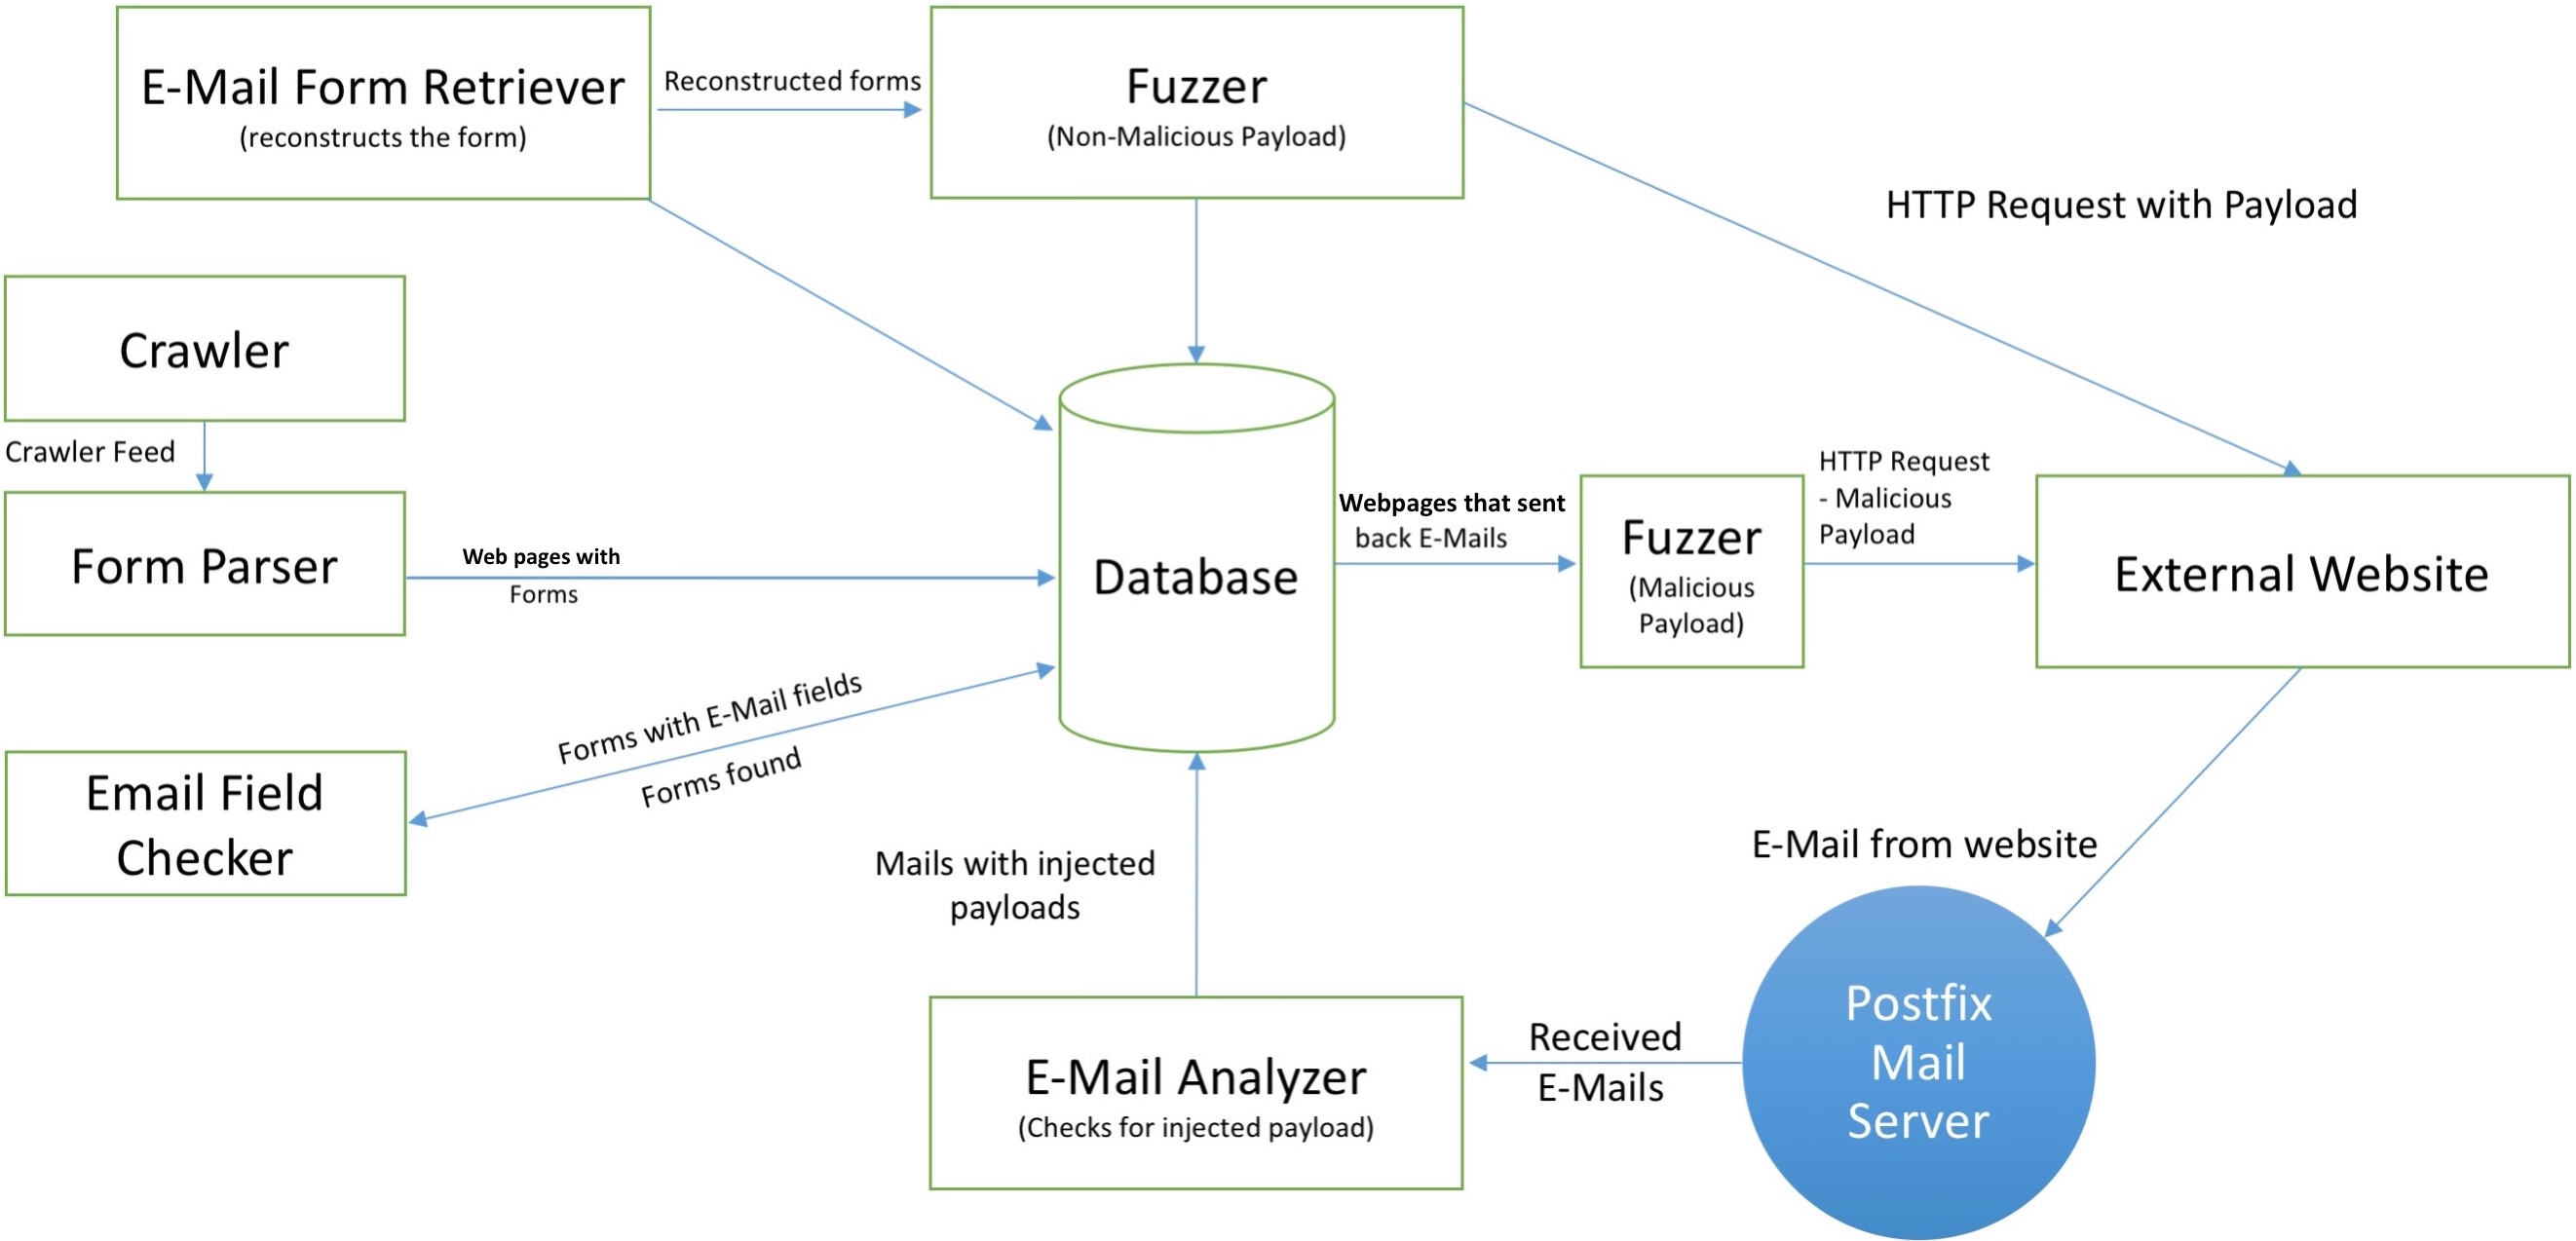
\includegraphics[width=.5\textwidth]{overall_crop}
	\caption{Overall system architecture.}
    \vspace{-5ex}
	\label{fig:overall}
\end{figure}

%\subsection{System Architecture}
\label{sys:arch}
Our system can be broadly divided into two modules: Data Gathering and Payload Injection.

The Data Gathering module is responsible for the following activities:
(1) Interface with the Crawler (Section~\ref{Comp:Crawler}) and
receive the URLs, (2) Parse the HTML for the corresponding URL and
store the relevant form data (Section~\ref{Comp:FP}), and (3) Check
for the presence of HTML forms that could allow a user to send/receive
\email and store references to these forms (Section~\ref{Comp:EMFC}).

    
The Payload Injection module is responsible for the following
activities: (1) Retrieve the HTML forms that could allow a user to
send/receive \email and reconstruct these forms
(Section~\ref{Comp:EMFR}), (2) Inject these forms with benign data
(non-malicious payloads) and generate an HTTP request to the
corresponding URL (Section~\ref{Comp:Fuzzer}), (3) Analyze the
received \emails, extracting the \email header fields and checking for
the presence of the injected payloads (Section~\ref{Comp:EMA}), and
(4) Inject the HTTP requests that sent us \emails with malicious
payloads, and generate an HTTP request to the corresponding URL to
check if an \ehi vulnerability exists in that web application
(Section~\ref{Comp:Fuzzer}).

	%% The functionality of each component is discussed further in the `Components' section (Section~\ref{Comp}). The Payload Injection pipeline is not a linear, but cyclic process, as we inject different payloads and analyze the received \emails.


\subsection{System Components}

\label{Comp}
\label{Comp:Crawler}
\label{Comp:EMFR}
\label{Comp:Fuzzer}
\label{Comp:EMA}
The Data Gathering module and Payload Injection modules are composed of smaller components. This section describes the functionality of those components.

\subsubsection{Data Gathering}
We used an open-source Apache Nutch based Crawler~\cite{nutch}. The \texttt{Crawler} provides the system with a continuous feed of URLs and the HTML contained in those pages. 
\label{Comp:FP}
The \texttt{Form Parser} is responsible for parsing the HTML and retrieving data about the HTML
forms on the page, including the following: (1) Form attributes, such
as \texttt{method} and \texttt{action} (URL) for the HTTP request, (2)
Data about form inputs, such as their attributes, names, and
default values. The default values are essential for fields like
{\lstinline{<input type="hidden">}} as these fields are usually used
to check for the submission of forms by bots, and (3) Presence of the {\lstinline{<base>}} element in the HTML, as this affects the final URL to which the form is to be submitted (if the \texttt{action} attribute is a relative URL).

\label{Comp:EMFC}
The \texttt{\Email Field Checker} is the final stage in the Data Gathering module. It receives the HTML form data and checks for the presence of \email fields in those forms. If any \email fields are found, it stores references to these forms.
The intuition here is that we do not want to try to fuzz all HTML forms on the web to look for \ehi vulnerabilities, rather just those HTML forms that are likely to invoke server-side email functionality.

The \Email Field Checker searches for the words \texttt{e-mail},
\texttt{mail} or \texttt{email} within the form, instead of an
explicit HTML5 \email field (e.g.,\ {\lstinline{<input type="email">}}). This is by design, taking into account a common
design pattern used by web developers, where they may have a text
field with an \texttt{id} or \texttt{name} attribute set to
\texttt{email}, instead of an actual \email type attribute, for
purposes of backward compatibility with older browsers. The output of this stage is stored in the database and acts as the input to the Payload Injection module.

%% Compared to searching for explicit \email fields, by searching for the presence of the words \texttt{\email}, \texttt{mail} or \texttt{email} in the form, we are assured very few false negatives. This is because our system is bound to find \email fields with their \texttt{type}, \texttt{name}, or \texttt{id} set to one of these words. The system is also substantially faster as we do not have to parse the individual form fields at this point in the pipeline. However, despite the advantages, this might also lead to a false positive rate. We discuss this possibility in detail in Section~\ref*{issues:fpr} - Design Issues.
\textbf{\Email Form Retriever} is the first stage in the Payload Injection
module. It does the following: (1) Retrieve forms and
remove duplicates, (2) reconstruct
each form's input fields and values from stored form data, and (3) construct the target URL
to create an HTTP request for fuzzing.

\textbf{Fuzzer}
% Adam: we should call these something else but modules. We already have the top two modules, which are composed of components, now we need to split these into something (not components again). - DONE
interacts directly with the external web applications. The system
injects payloads in two stages to reduce the total number of HTTP requests the system generates to detect an \ehi vulnerability. Making HTTP requests is an expensive process~\cite{httpperf}, and can cause bottlenecks in a Crawler-Fuzzer system~\cite{ShkapenyukTorstenSuel2001}.
The two different payloads used for fuzzing are:

\noindent\textbf{Non-Malicious Payload.}
The non-malicious payload is simply an \email address. The goal is to see if the web application will send an \email message based on our input. The specific format of the \email is \lstinline|reguser#@example.com|, where \texttt{\#} is replaced by an internal id that uniquely maps the payload to the form, and \texttt{example.com} is replaced by our domain.

\noindent\textbf{Malicious Payload.}
After receiving an \email from a specific form, we use the malicious payload to try to exploit an \ehi vulnerability. We inject the form fields with the \texttt{bcc} (blind carbon copy) header. If the vulnerability is present, this will cause the server to send a copy of the \email to the \email address we added as the \texttt{bcc} field.

We consider a special case: the addition of an \texttt{x-check:in} header field to the payloads. This is due to Python's exhibited behavior when attaching
headers. Instead of overwriting a header if it is already present, Python will ignore duplicate headers. So, if the \texttt{bcc} field is already present as part of the headers, our injected \texttt{bcc} header would be ignored. To overcome this, we inject a new header that is not likely to be generated by the web application. 

We created four different malicious payloads. Each of these payloads
is crafted for a particular use case. The four payloads are:
(1) nuser\#@example.com\textbackslash{}n\-bcc:\-maluser\-\#\-@example.com,
(2) nuser\#@\-example.com\textbackslash{}n\-bcc:\-maluser\-\#\-@example.com\textbackslash{}n\-x-check:in,
(3) nuser\#@\-example.com\textbackslash{}r\textbackslash{}n\-bcc:\-maluser\#\-@example.com,
and (4) nuser\#\-@example.com\-\textbackslash{}r\textbackslash{}n\-bcc:\-maluser\#\-@example.\-com\textbackslash{}r\textbackslash{}n\-x-check:in.
	
Payload 1 is the most minimal payload: it injects a newline character followed by the \texttt{bcc} field. Payload 2 contains the additional \texttt{x-check} header to inject Python-based web applications. Payloads 3 and 4 are added for purposes of cross-platform fuzzing: \texttt{\textbackslash{}r\textbackslash{}n} is the ``Carriage Return - New Line (CRLF)'' used on Windows systems~\cite{rfc2616}. The \# are replaced by an internal id, for mapping to the forms.

% Adam: If we need to cut things for space, we can cut this next line and the payload coverage table.

%\begin{table}[tbp]
%	\centering
%	\normalsize
%	\begin{tabular}{|c|c|c|}
%		\hline
%		\multicolumn{1}{|c|}{\textbf{Payload}} & \multicolumn{1}{c}{\textbf{Languages covered}} & \multicolumn{1}{|c|}{\textbf{Platforms covered}}\\
%		\hline
%		1 & PHP, Java, Ruby, etc. & Unix\\
%		\hline
%		2 & PHP, Java, Ruby, etc. & Windows\\
%		\hline
%		3 & Python & Unix\\
%		\hline
%		4 & Python & Windows\\
%		\hline
%	\end{tabular}
%	\caption[\titlecap{Payload coverage}]{Payload coverage, each payload covers a different platform/language.}
%	\label{tab:payloadcov}
%\end{table}

%% \begin{table}[tbp]
%% 	\centering
%% 	\scriptsize
%% 	\begin{tabular}{|c|c|c|}
%% 		\hline
%% 		\multicolumn{1}{|c|}{\textbf{Language/Platform}} & \multicolumn{1}{c}{\textbf{Unix}} & \multicolumn{1}{|c|}{\textbf{Windows}}\\
%% 		\hline
%% 		\textbf{PHP, Java, Ruby} & 1 & 3\\
%% 		\hline
%% 		\textbf{Python} & 2 & 4\\
%% 		\hline
%% 	\end{tabular}
%% 	\caption[\titlecap{Payload coverage}]{Payload coverage, each payload covers a different platform/language.}
%% 	\label{tab:payloadcov}
%% \end{table}

Along with the payload, the Fuzzer also injects data into the other fields of the form. This data must pass validation constraints on the individual input fields (e.g.,\ name field might not be allow numbers).  As crawling and fuzzing input fields on the web is an open problem~\cite{raghavan2000crawling}, we chose to go with a best-effort approach. To maximize the amount of vulnerabilities the system discovers, the data injected into the input fields should adhere to the constraints. The Fuzzer uses a ``Data Dictionary'' which has predefined ``keys'' and ``values'' for standard input fields such as \texttt{name}, \texttt{date}, \texttt{username}, \texttt{password}, \texttt{text}, and \texttt{submit}.
The values for these are generated for each form, based on generally followed guidelines for such fields. For example, password fields should consist of at least one uppercase letter, one lowercase letter, and special characters.

When the fuzzed data is ready, the Fuzzer constructs the appropriate HTTP request (GET or POST) and sends the HTTP request to the URL that was generated by the \Email Form Retriever (Section~\ref{Comp:EMFR}). 


\textbf{Injection Verification}
module checks for the presence of injected data in the received \emails. This module works on the \emails received and stored by our Postfix server, and, depending on the user account that received the \email, it performs different functions.

\noindent\textbf{Analyzing regular e-mail.}
\sloppy
`Regular \email' refers to the \emails received by account {\lstinline{reguser#@example.com}} that were sent due to injecting the regular, non-malicious, payload (discussed in Section~\ref{Comp:Fuzzer}). The objective of the analysis on this \email is identify if the input fields that we injected with data appear on the resulting \email, and if so, which fields appear where.

To find this, we parse each received \email, and check whether \emph{any} of the fields we injected with data appear in either the headers or body of the \email. These could be fields such as name, username, age, etc. If they do, we add them to the list of fields that can \emph{potentially} result in an \ehi vulnerability for the given \email. 

We then pass on this information back to the Fuzzer pipeline, along with the vulnerable form, where these fields are \emph{also} fuzzed along with the \email fields to check for the presence of \ehi.

\noindent\textbf{Analyzing \email with payloads}
The ``\emails with payloads'' refers to \emails received by either the {\lstinline{nuser#@example.com}} or {\lstinline{maluser#@example.com}} accounts. These \emails could only be received as a result of injecting the malicious payloads that were discussed in Section~\ref{Comp:Fuzzer}. 

\noindent\textbf{Detecting injected \texttt{bcc} headers}
As discussed in the payloads Section~(\ref{Comp:Fuzzer}), the payloads were crafted such that the \emails received by the \texttt{maluser} account directly indicate the presence of the injected \texttt{bcc} field. 

\label{analyze:detect_x_check}
\noindent\textbf{Detecting injected \texttt{x-check} headers} \Emails
not received by the \texttt{maluser} account but by the \texttt{nuser}
account constitute a special category of \emails. These \emails could
have been generated due to two reasons: (1) The web application
performed sanitization and stripped out the \texttt{bcc}
part of the payload, thereby sending \emails only to the
\texttt{nuser} account. These \emails then act as proof that the
vulnerability was not found on the given URL. (2) The \texttt{bcc}
header can be ignored for other reasons (e.g.,\ Python's default
behavior when it encounters duplicate headers). In this case, we check
if the \email contains the custom header \texttt{x-check}. If it does,
then this is a successful exploit of the vulnerability.



%	\section{Validation}

%Our system was run on a server with the following configuration: Dell
PowerEdge T110 II Server, CPU: Intel(R) Xeon(R) CPU E3-1220 V2 @
3.10GHz, Cache Size: 8,192 KB, No. of Cores : 4, Total Memory (RAM) : 16 GB.

To validate our system, we constructed three sets of web applications in PHP, Python, and Ruby. Each of these applications was a simple web application that accepted user input to construct and send an \Email.

The server-side code for PHP is shown in Listings~\ref{code:phpemi},
while the Python and Ruby code is not shown for space limitations.

% Adam: I think it might be nice to have the Ruby code here too. - DONE.

Before performing a wide scan of the web, we verified that our system was able to detect the \ehi vulnerabilities present in all the sample web applications. 

%% We tested for the headers being injected in real-time by running an instance of MailCatcher, set to listen on all SMTP messages. A sample screenshot of a fuzzed request for the Ruby backend (generated in PostMan) is shown in Figure~\ref{fig:postmanruby}. The \email sent due to injecting this payload (as captured by MailCatcher) is shown in Figure~\ref{fig:mailcatcherruby}. It can be seen that the headers have been added to the resulting \email, and we have successfully managed to overwrite the \texttt{Subject} field with our message, `hello'.

%% The astute reader might have noticed that in the given example we have used \texttt{\%0a} to separate the headers, while in Section~\ref{Comp:Fuzzer}, we had used \texttt{\textbackslash{}n}. This is due to URL encoding~\cite{rfc1738}, wherein special characters in th URL are `encoded' or `escaped' with their ASCII equivalent.
%% The reason why we do not have to do this with the payloads our system injects is due to the fact that the Python Requests library that we use to generate the HTTP requests automatically does this encoding for us.

%% \begin{lstlisting}[language=HTML,caption={HTML page for showcasing
%%       \ehi, a simple front-end for our
%%       examples.},label={code:html}, float]
%% <!doctype html>
%% <html lang="en">
%% <head>
%% <meta charset="utf-8">
%% <meta name="author" content="XYZ">
%% <title>Mock Email</title>
%% </head>
%% <body>
%% <form action="script-path" method="post">
%% <input type="text" name="email">
%% <textarea name="msg"></textarea>
%% <input type="submit" value="Email Me!">
%% </form></body></html>
%% \end{lstlisting}
%\begin{lstlisting}[language=Ruby,caption={Ruby program with e-mail
      header injection vulnerability.},label={code:rubyemi}, float]
require 'sinatra'
require 'net/smtp'
get '/hello' do
email = params[:email]
message = """
    From: Sch <sch@example.com>
    Subject: SMTP e-mail test
    To: #{email}

    This is a test e-mail message.
"""
Net::SMTP.start('localhost',1025) do |smtp|
smtp.send_message message, 'sch@example.com', 'to@todomain.com'
end
end
\end{lstlisting}


%% \begin{figure}[tbp]
%% 	\centering
%% 	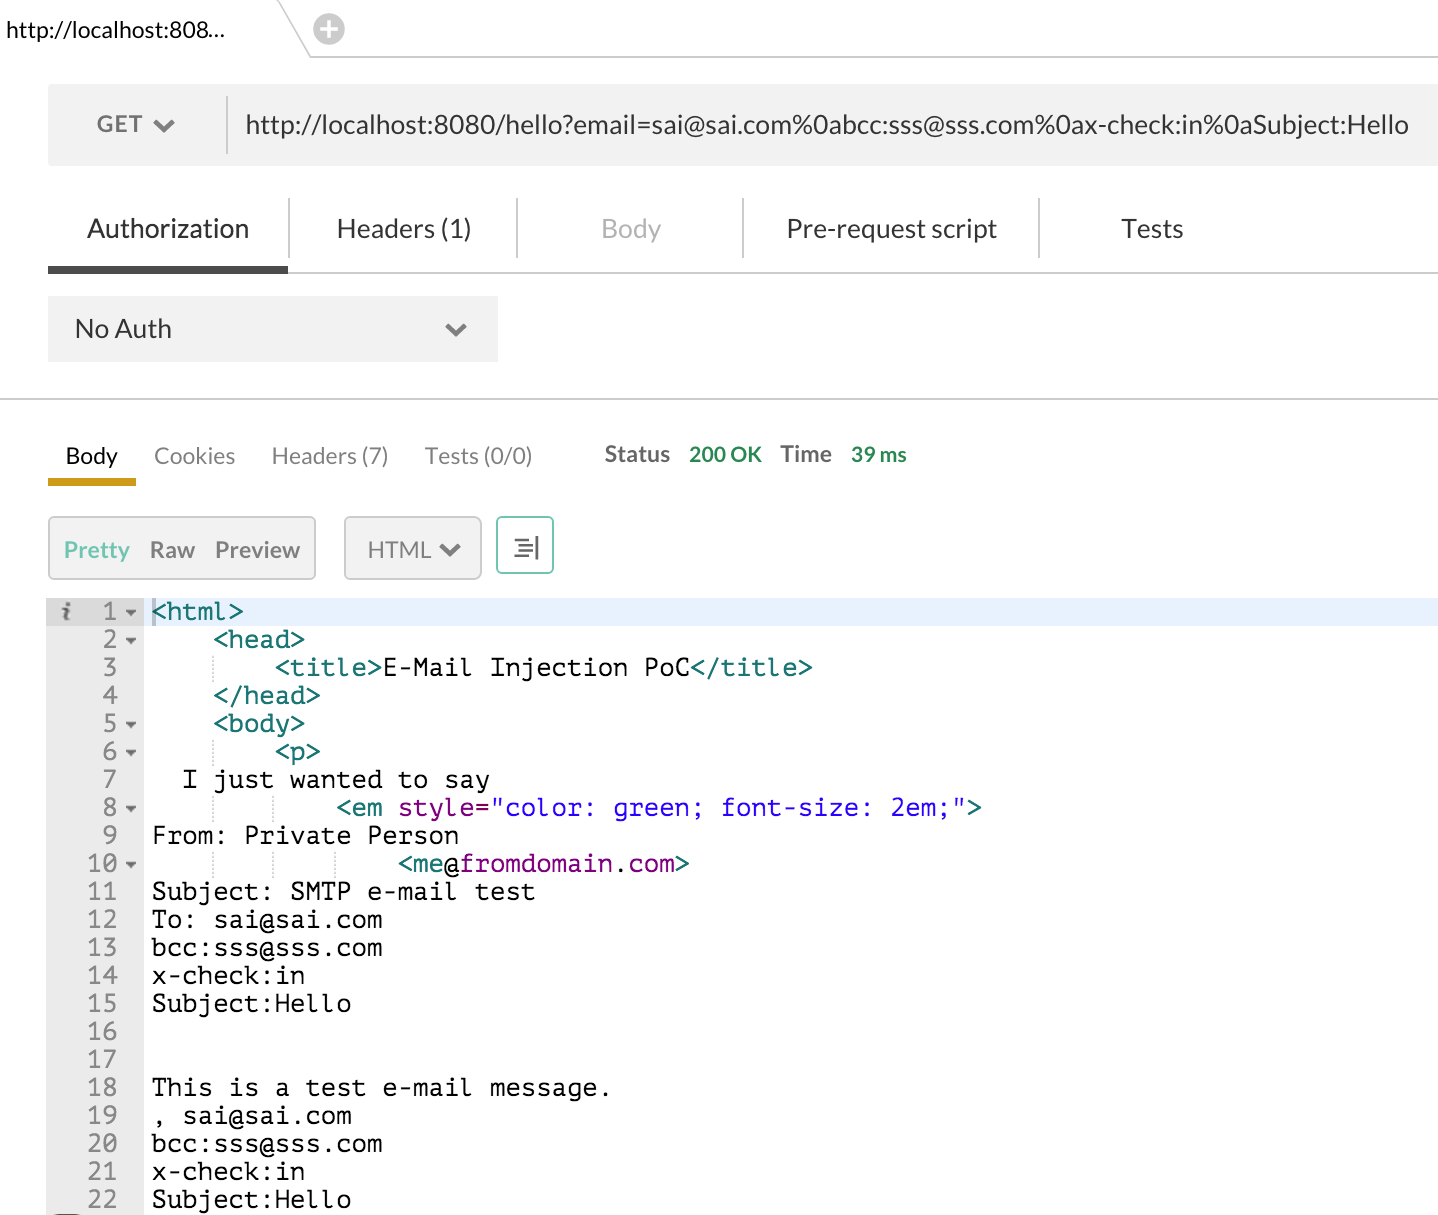
\includegraphics[width=\linewidth]{System/EMI_Postman_Ruby}
%% 	\caption[\titlecap{Fuzzing a request for the Ruby backend}]{Fuzzing a request for the Ruby backend, the payload can be seen inside the address bar.}
%% 	\label{fig:postmanruby}
%% \end{figure}

%% \begin{figure}[tbp]
%% 	\centering
%% 	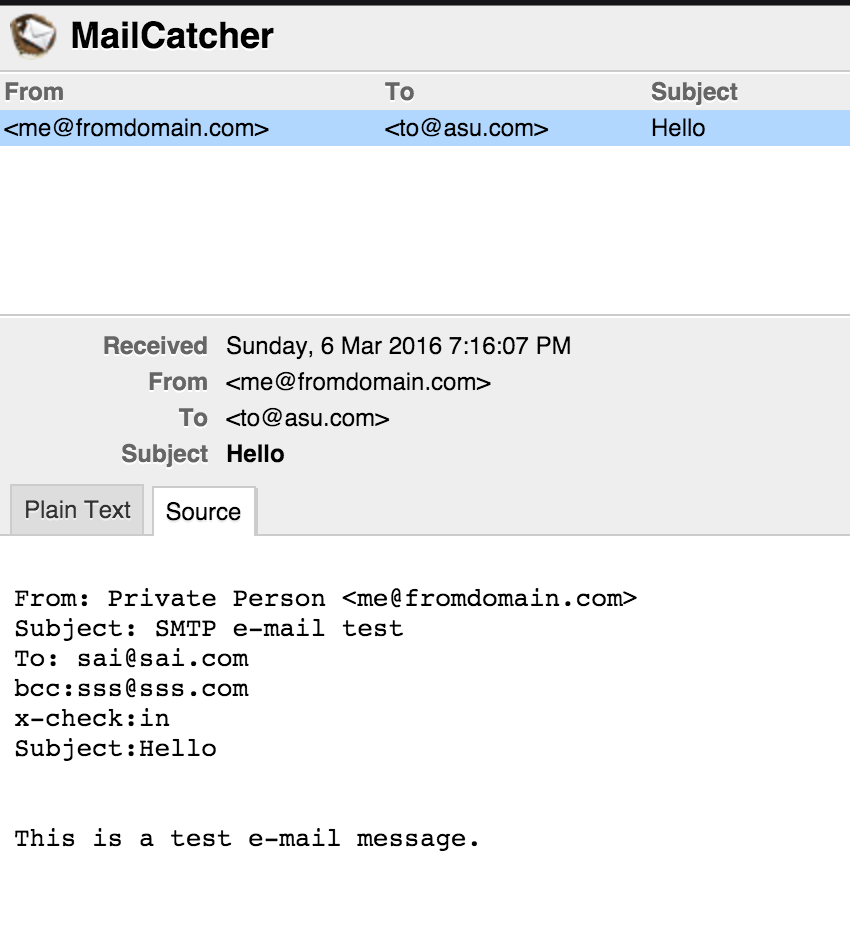
\includegraphics[width=\linewidth]{System/EMI_Mailcatcher_Ruby}
%% 	\caption[\titlecap{\Email Header Injection proof of concept - Ruby}]{\Email header injection proof of concept - Ruby, we can see that multiple headers (bcc, x-check, subject) have been inserted into the resulting \email.}
%% 	\label{fig:mailcatcherruby}
%% \end{figure}


\section{Other Sections}\label{sec:Others}

Other sections are here. 


\section{Conclusion}\label{sec:Conclusion}

Conclusions are here.

%
\newpage
%
%
\section {Footnotes}
%
Footnotes within the text should be coded:
\begin{verbatim}
\footnote{Text}
\end{verbatim}
{\itshape Sample Input}
\begin{flushleft}
Text with a footnote\verb|\footnote{The |{\tt footnote is automatically
numbered.}\verb|}| and text continues \dots
\end{flushleft}
{\itshape Sample Output}
\begin{flushleft}
Text with a footnote\footnote{The footnote is automatically numbered.}
and text continues \dots
\end{flushleft}
%

\section{Tables}
%
Table captions should be treated
in the same way as figure legends, except that
the table captions appear {\itshape above} the tables. The tables
will be numbered automatically.
%
\subsection{Tables Coded with \protect\LaTeX{}}

\medskip\noindent{\itshape Sample Output}
\begin{table}
\caption{Critical $N$ values}
\begin{center}
\renewcommand{\arraystretch}{1.4}
\setlength\tabcolsep{3pt}
\begin{tabular}{llllll}
\hline\noalign{\smallskip}
${\mathrm M}_\odot$ & $\beta_{0}$ & $T_{\mathrm c6}$ & $\gamma$
  & $N_{\mathrm{crit}}^{\mathrm L}$
  & $N_{\mathrm{crit}}^{\mathrm{Te}}$\\
\noalign{\smallskip}
\hline
\noalign{\smallskip}
 30 & 0.82 & 38.4 & 35.7 & 154 & 320 \\
 60 & 0.67 & 42.1 & 34.7 & 138 & 340 \\
120 & 0.52 & 45.1 & 34.0 & 124 & 370 \\
\hline
\end{tabular}
\end{center}
\end{table}

% adding bibliography here, apparently LNCS prefers inline instead of .bib
\bibliographystyle{splncs03}
\bibliography{biblio}
\end{document}
